\paragraph{Colour Choice}

In the software, some colours have been chosen to make the software more appealing to the user. When these colours have been chosen, it has been important that the colour give the right statement, and that they seem attractive to the user.

The colours were chosen by using an online tool called Paletton\cite{paletton}, which suggests a colour theme based on the colours the user choose. Similar tools are available online, though Paletton was easy to use and did not require any knowledge about the program before using it.

The colour for the software that was discussed first was a red colour. This was supposed to be the colour of headlines and such in the software. The reason for discussing red is that red indicates appetite and food\cite{color_psychology}. Red was not chosen though, as it is too strong of a colour, and this might put the user off. Red can also indicate danger or alerts, so choosing this colour might confuse some users and make them think that what they are doing is wrong.

Since red was not the optimal choice of colour, orange was considered for it's similarity to red. Orange has the same quality of red of encouraging appetite for the user. Orange is also a cheerful colour, and it was found to be very appealing, and it could be used in the program without standing out too much, or giving the user wrong impressions.

\begin{figure}[H]
	\centering
    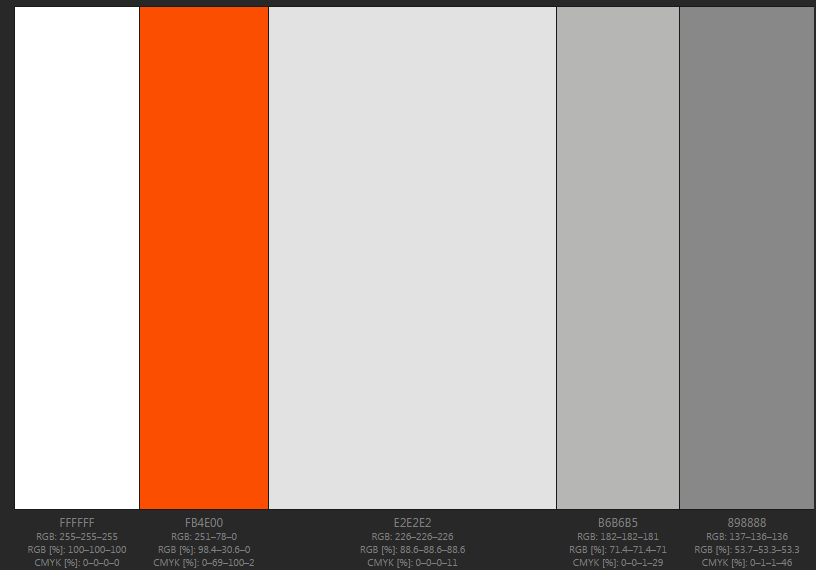
\includegraphics[width=0.9\textwidth]{Grafik/FoodPlanner/ChosenColours}
	\caption{The chosen colours for the software}
	\label{ChosenColours}
\end{figure}

The shade of orange that was chosen, and the colours that matched according to Paletton can be seen in \cref{ChosenColours}.

The colour \#898888 is used for the borders of the program. If something is parted, or a button needs a border, this colour is used. The reason for choosing this colour is that it is much darker than the other colours and gives a clear indication of an ending item.

The colour \#FB4E00 is the orange colour as can be seen in \cref{ChosenColours}. This colour is the one used for the headline text, as is the main colour of the program, since it is the only colour that can't be characterized as a neutral colour. It is only used for the headline text, as it would be difficult for the user to read the text if it was all orange.

The colour \#E2E2E2 is used for the background of the software. This is a very light colour, and it is easy to read black text of it, and the orange headlines can be seen. Therefore this colour was chosen for the background. The white colour \#FFFFFF was also considered, but it was too light, and might irritate the user, and it did not go as well with the borders as \#E2E2E2.

